\chapter{Interplay between Larval Trait Parameters}
In the base model of larval stage, trait parameters used are initial feeding rate, efficiency, critical size and waste tolerance. These parameters can not be measured directly via experimental approaches, but their effect on other larval traits such as body size, feeding rate at the third instar, development time can be measured easily. Here, I explore how larval trait parameters interact with each other and affect body size, time to reach critical size, feeding rate at critical size and survivorship. Since feeding rate in the model stays constant after reaching critical size, it can be taken as proxy for feeding rate at the third instar stage.

\section{Initial Feeding Rate and Efficiency}
In MB culture (low density), fig ~\ref{fig:fr vs eff mb} shows having higher efficiency as well as higher initial feeding rate gives higher larval body size, but lower time to reach critical size. Feeding rate at critical size is dependent on time taken to reach critical size which is dependent on body size increment at each time step. This body size increment is proportional to the current feeding rate and efficiency. Thus, efficiency and initial feeding rate both affect the feeding rate shown at the critical size. Having lower efficiency and higher initial feeding rate tends to give higher feeding rate at critical size in MB culture. Survivorship does not show any pattern at low density, since most of the larvae are competing very less and are able to survive easily. \\
\begin{figure}[h]
\subfloat[MB culture]{
  \centering
  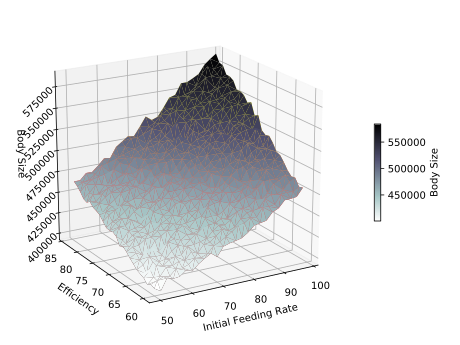
\includegraphics[trim = 0 0 150 50, clip, width=.33\columnwidth]{C3/Figs/fr_eff/fr_eff_bs_MB}
}
\subfloat[MCU culture]{
  \centering
  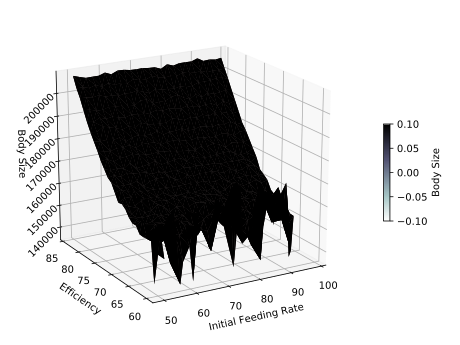
\includegraphics[trim = 0 0 150 50, clip, width=.33\columnwidth]{C3/Figs/fr_eff/fr_eff_bs_MCU}
}
\subfloat[CCU culture]{
  \centering
  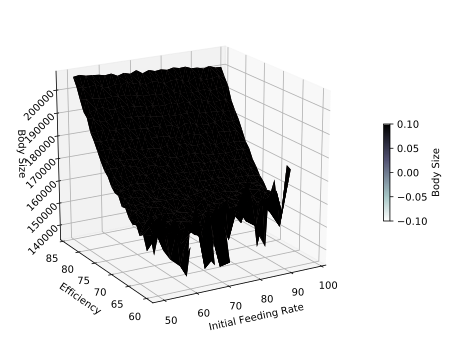
\includegraphics[trim = 0 0 150 50, clip, width=.33\columnwidth]{C3/Figs/fr_eff/fr_eff_bs_CCU}
}
\caption{Effect of initial feeding rate and efficiency on body size at different larval densities}
\label{fig:fr_eff_bs}
\end{figure}

\begin{figure}[h]
\subfloat[MB culture]{
  \centering
  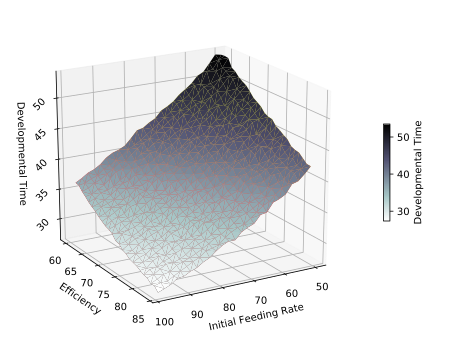
\includegraphics[trim = 0 0 150 50, clip, width=.33\columnwidth]{C3/Figs/fr_eff/fr_eff_dt_MB}
}
\subfloat[MCU culture]{
  \centering
  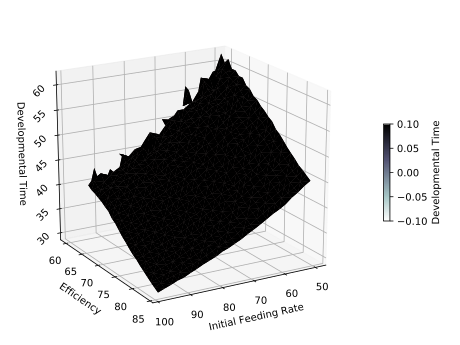
\includegraphics[trim = 0 0 150 50, clip, width=.33\columnwidth]{C3/Figs/fr_eff/fr_eff_dt_MCU}
}
\subfloat[CCU culture]{
  \centering
  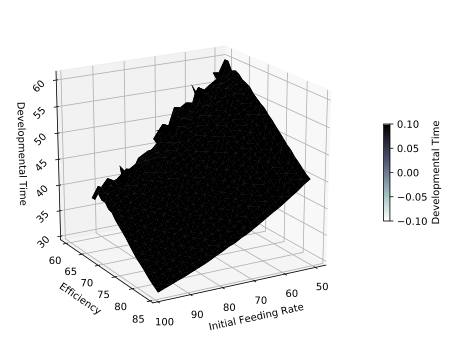
\includegraphics[trim = 0 0 150 50, clip, width=.33\columnwidth]{C3/Figs/fr_eff/fr_eff_dt_CCU}
}
\caption{Effect of initial feeding rate and efficiency on developmental time}
\label{fig:fr_eff_dt}
\end{figure}\\ \\

\begin{figure}[h]
\subfloat[MB culture]{
  \centering
  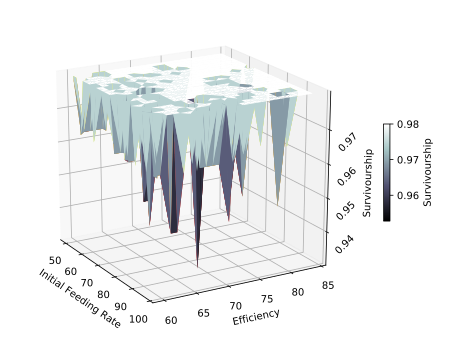
\includegraphics[trim = 0 0 150 50, clip, width=.33\columnwidth]{C3/Figs/fr_eff/fr_eff_sur_MB}
}
\subfloat[MCU culture]{
  \centering
  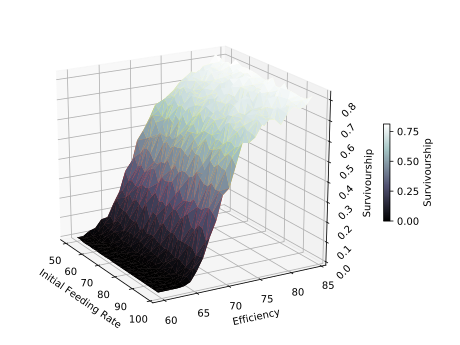
\includegraphics[trim = 0 0 150 50, clip, width=.33\columnwidth]{C3/Figs/fr_eff/fr_eff_sur_MCU}
}
\subfloat[CCU culture]{
  \centering
  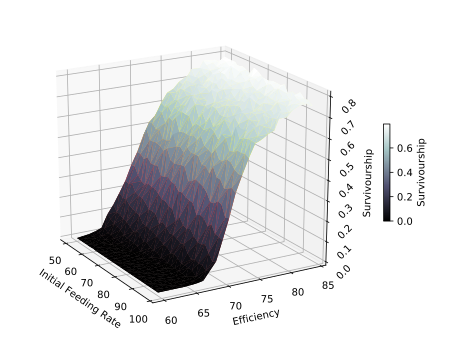
\includegraphics[trim = 0 0 150 50, clip, width=.33\columnwidth]{C3/Figs/fr_eff/fr_eff_sur_CCU}
}
\caption{Effect of initial feeding rate and efficiency on survivorship}
\label{fig:fr_eff_sur}
\end{figure}

\begin{figure}[h]
\subfloat[MB culture]{
  \centering
  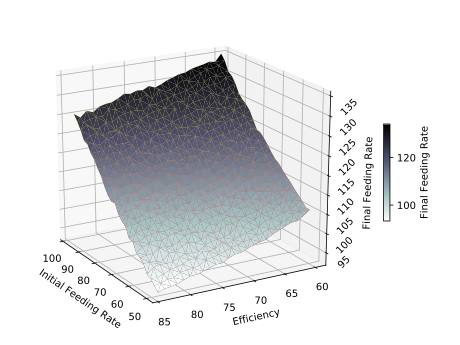
\includegraphics[trim = 0 0 150 50, clip, width=.33\columnwidth]{C3/Figs/fr_eff/fr_eff_frt_MB}
}
\subfloat[MCU culture]{
  \centering
  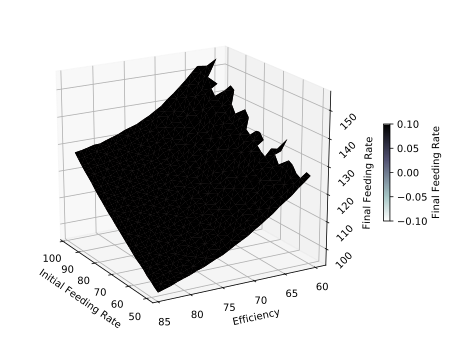
\includegraphics[trim = 0 0 150 50, clip, width=.33\columnwidth]{C3/Figs/fr_eff/fr_eff_frt_MCU}
}
\subfloat[CCU culture]{
  \centering
  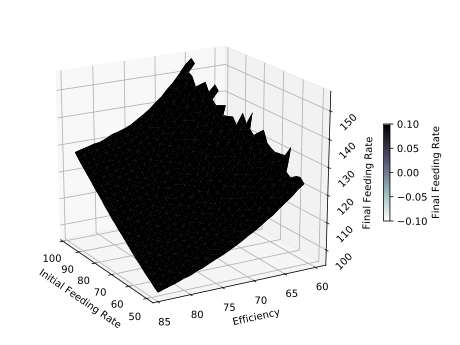
\includegraphics[trim = 0 0 150 50, clip, width=.33\columnwidth]{C3/Figs/fr_eff/fr_eff_frt_CCU}
}
\caption{Effect of initial feeding rate and efficiency on final feeding rate}
\label{fig:fr_eff_frt}
\end{figure}
In MCU and CCU cultures (high densities), fig ~\ref{fig:fr vs eff mcu} and fig ~\ref{fig:fr vs eff ccu} show that time to reach critical size show similar pattern as seen in MB culture with varying efficiency and initial feeding rate. The maxima possible is higher in high density cultures than maxima possible in low density culture, showing that it takes more time to reach given critical size at high densities than at low density with same efficiency and initial feeding rate values. Feeding rate shown at critical size also shows similar pattern as seen in MB culture but with higher maxima reached with same parameter ranges. This suggests feeding rate shown at critical size is also a density dependent trait.The complete white pixels in all heatmaps (fig ~\ref{fig:fr vs eff mcu} and fig ~\ref{fig:fr vs eff ccu}) are the values where none of the larvae survived, so the trait could not be measured and are to be excluded.
\\ \\
At high densities, especially at MCU density, body size and survivorship are not affected by initial feeding rate, unlike at low density. Food acquired while having either higher or lesser initial feeding rate, remains almost the same. This is due to the decrease in food quality is higher for higher initial feeding rate. Thus, overall body size increment which is majorly determined by food quality at high densities, is approximately same in both cases i.e. larval growth with both higher and lower initial feeding rate. Survivorship also shows similar pattern as body size for these two parameters, since it is determined by whether critical size is reached or not.\\ \\
\begin{figure}[!tbp]
  \centering
  \includegraphics[width=0.75\textwidth]{C3/Figs/Feeding_rate_vs_Efficiency_MCU}
  \caption{Effect of initial feeding rate and efficiency on larval traits in MCU culture}
  \label{fig:fr vs eff mcu}
  \vspace{24pt}
  \includegraphics[width=0.75\textwidth]{C3/Figs/Feeding_rate_vs_Efficiency_CCU}
  \caption{Effect of initial feeding rate and efficiency on larval traits in CCU culture}
  \label{fig:fr vs eff ccu}
\end{figure}
\newpage

\section{Initial Feeding Rate and Critical Size}
In MB culture, fig ~\ref{fig:fr vs cs mb} shows having higher critical size and higher initial feeding rate leads to higher larval body size. Lower critical size and higher initial feeding rate is beneficial in having lower time to reach critical size. Feeding rate at critical size is majorly determined by initial feeding rate, while having higher critical size gives slightly higher feeding rate, since time to reach critical size is more. Survivorship is not affected by either initial feeding rate or critical size at low density, since competition for food is minimal. \\ \\
\begin{figure}
  \centering
  \includegraphics[width=0.75\textwidth]{C3/Figs/Critical_size_vs_Feeding_rate_MB}
  \caption{Effect of initial feeding rate and critical size on larval traits in MB culture}
  \label{fig:fr vs cs mb}
\end{figure}\\
In MCU culture fig ~\ref{fig:fr vs cs mcu}, body size is not affected by either critical size or initial feeding rate and post-critical growth is very less. Time to reach critical size and feeding rate at critical size show similar pattern as shown in MB culture with higher maxima for same values. Survivorship is only affected by critical size and initial feeding rate has no effect on survivoship at MCU density. Lower critical size shows trend for higher survivoship, since larvae are able to pupate in lesser time before food quality decreases drastically.\\ \\
\begin{figure}[!tbp]
  \centering
  \includegraphics[width=0.75\textwidth]{C3/Figs/Critical_size_vs_Feeding_rate_MCU}
  \caption{Effect of initial feeding rate and critical size on larval traits in MCU culture}
  \label{fig:fr vs cs mcu}
  \vspace{24pt}
  \includegraphics[width=0.75\textwidth]{C3/Figs/Critical_size_vs_Feeding_rate_CCU}
  \caption{Effect of initial feeding rate and critical size on larval traits in CCU culture}
  \label{fig:fr vs cs ccu}
\end{figure}\\\\
In CCU culture, fig ~\ref{fig:fr vs cs ccu}, patterns of body size, time to reach critical size and feeding rate at critical size similar to the ones in MCU culture. Survivorship shows small effect of initial feeding rate as well along with critical size. Having lesser average initial feeding rate in the population leads to slower urea build up and decrease in food quality of the feeding band, thus larvae with higher critical size are able to survive.
\section{Critical Size and Efficiency}
In MB culture, fig ~\ref{fig:cs vs eff mb}, shows increase in body size with increase in critical size and efficiency. Feeding rate at critical size and time to reach critical size both increase with increasing critical size and decreasing efficiency. Higher efficiency leades to decrease in critical size thus feeding rate shown at critical size reaches lesser maxima. Survivorship shiws no effect of these parameters at low density.\\ \\
\begin{figure}[ht]
  \centering
  \includegraphics[width=0.75\textwidth]{C3/Figs/Critical_size_vs_Efficiency_MB}
  \caption{Effect of critical size and efficiency on larval traits in MB culture}
  \label{fig:cs vs eff mb}
\end{figure}\\
\begin{figure}[!tbp]
  \centering
  \includegraphics[width=0.75\textwidth]{C3/Figs/Critical_size_vs_Efficiency_MCU}
  \caption{Effect of critical size and efficiency on larval traits in MCU culture}
  \label{fig:cs vs eff mcu}
  \vspace{24pt}
  \includegraphics[width=0.75\textwidth]{C3/Figs/Critical_size_vs_Efficiency_CCU}
  \caption{Effect of critical size and efficiency on larval traits in CCU culture}
  \label{fig:cs vs eff ccu}
\end{figure}\\\\
In MCU and CCU culture, fig ~\ref{fig:cs vs eff mcu} and fig ~\ref{fig:cs vs eff ccu}, all the larval traits show similar pattern as in MB density with critical size and efficiency. The maxima for feeding rate at critical size and time to reach critical size is higher compared to the ones at MB density. Body size and survivoship maxima are lesser at high density.
\pagebreak
